\chapter{Introducción específica} % Main chapter title

\label{Chapter2}

%----------------------------------------------------------------------------------------
%	SECTION 1
%----------------------------------------------------------------------------------------
En este capítulo se introduce la terminología de la red de comunicaciones del tren y del sistema de información visual al pasajero. Se presenta una descripción de la arquitectura del sistema y de sus módulos principales. También se introduce el sistema de carteles led que presentan información al pasajeros, en particular en los coches de las formaciones ferroviarias de Trenes Argentinos.\\

\section{Trenes: Red de comunicación TCN}

La red de comunicaciones del tren (TCN) sigue un estándar de la International Electrotechnical Commission (IEC) que presenta una arquitectura de buses jerárquicos de dos niveles que se pueden identificar en la figura 1: el bus de datos WTB y el MVB\cite{IEC-61375-1999}. El WTB se encarga de las comunicaciones entre coches a través de nodos con redundancia física, mientras que al bus MVB se conectan los dispositivos de cada coche. \\

\begin{figure}[ht]
	\centering
	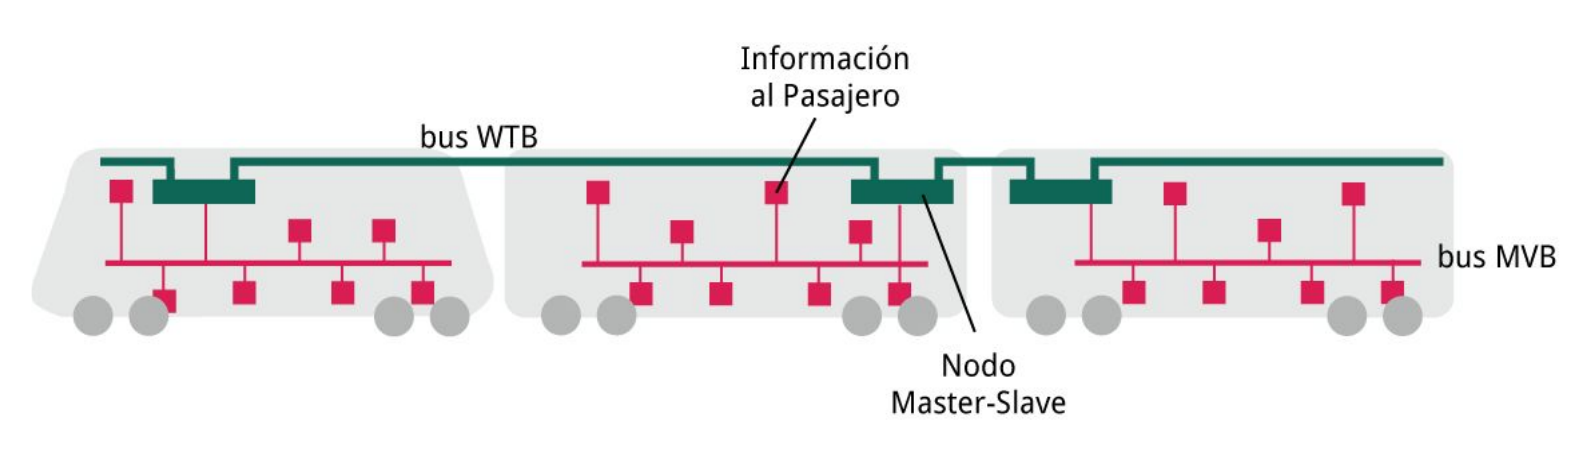
\includegraphics[width=1\textwidth]{./Figures/diagramaRedTCN.png}
	\caption{Diagrama del tren y de los buses WTB/MVB de la red TCN.}
	\label{fig:redTCN}
\end{figure}

Algunos de estos dispositivos o sistemas conectados al bus MVB son el control de puertas (DOORL/R), el aire acondicionado (HVAC), el sistema de tracción (VVVF), el sistema de control de frenos (BCU), entre otros. El mapa de recorrido y los carteles LED en conjunto con otros dispositivos como los parlantes y las cámaras de video (CCTV) forman un sistema denominado Sistema de información al pasajero (PIDS) que también se interconecta con el bus MVB. En la figura \ref{fig:sofseTCN} se presenta la topología de interconexión de sistemas de la red TCN de los trenes de SOFSE. Se puede observar la repetición de bloques funcionales en cada coche y , recuadrado en celeste, la ubicación en los coches cabecera del módulo PIDS.\\

\begin{figure}[h!]
	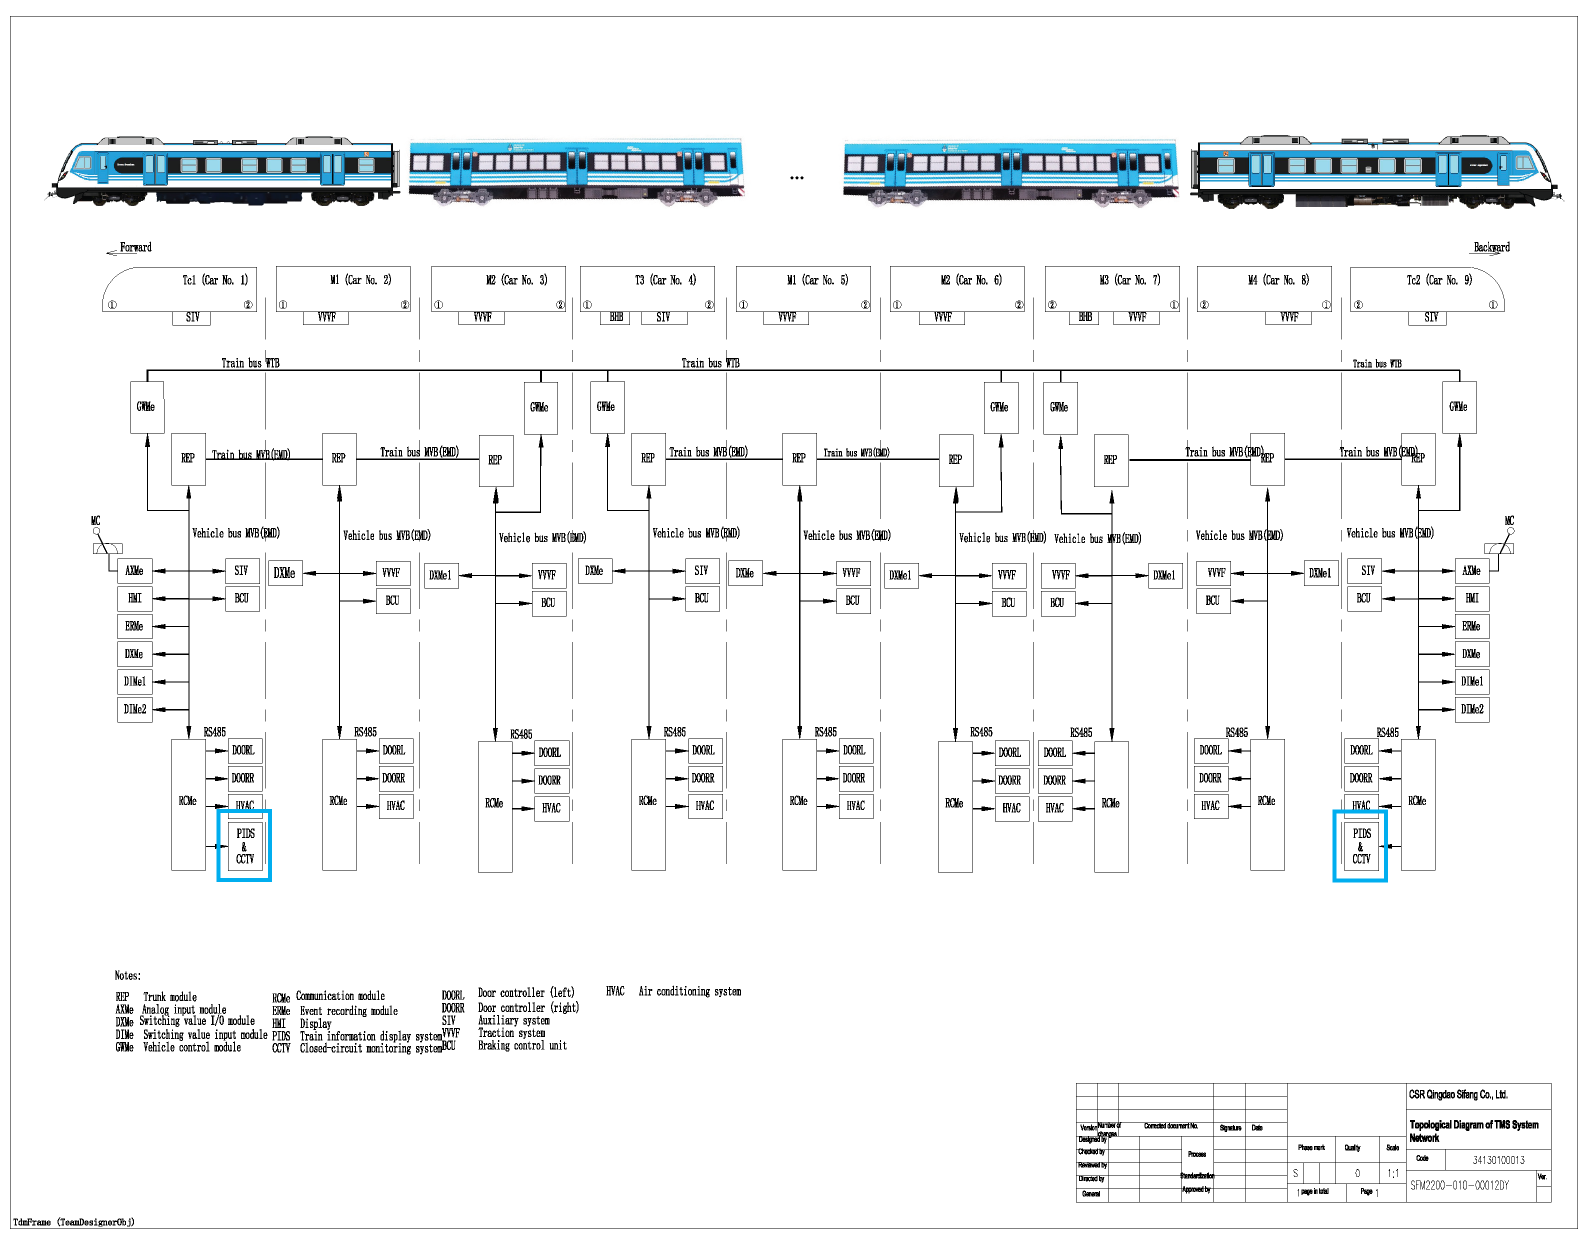
\includegraphics[width=1.4\textwidth, angle=90]{./Figures/diagramaTrenesArgentinosTCN.png}
	\caption{Diagrama de la red TCN de Trenes Argentinos. Plano cortesía SOFSE, editado por parte del autor.}
	\label{fig:sofseTCN}
\end{figure}

El bloque remarcado corresponde al sistema PIDS y al CCTV. Como se puede leer del plano, tal bloque se conecta a un módulo denominado RCMe a través de una red RS485. Este último bloque se corresponde uno a uno con un módulo de hardware instalado en los rack de salón, indicado en la figura \ref{fig:imgRackTCN}. \\

\begin{figure}[ht]
	\centering
	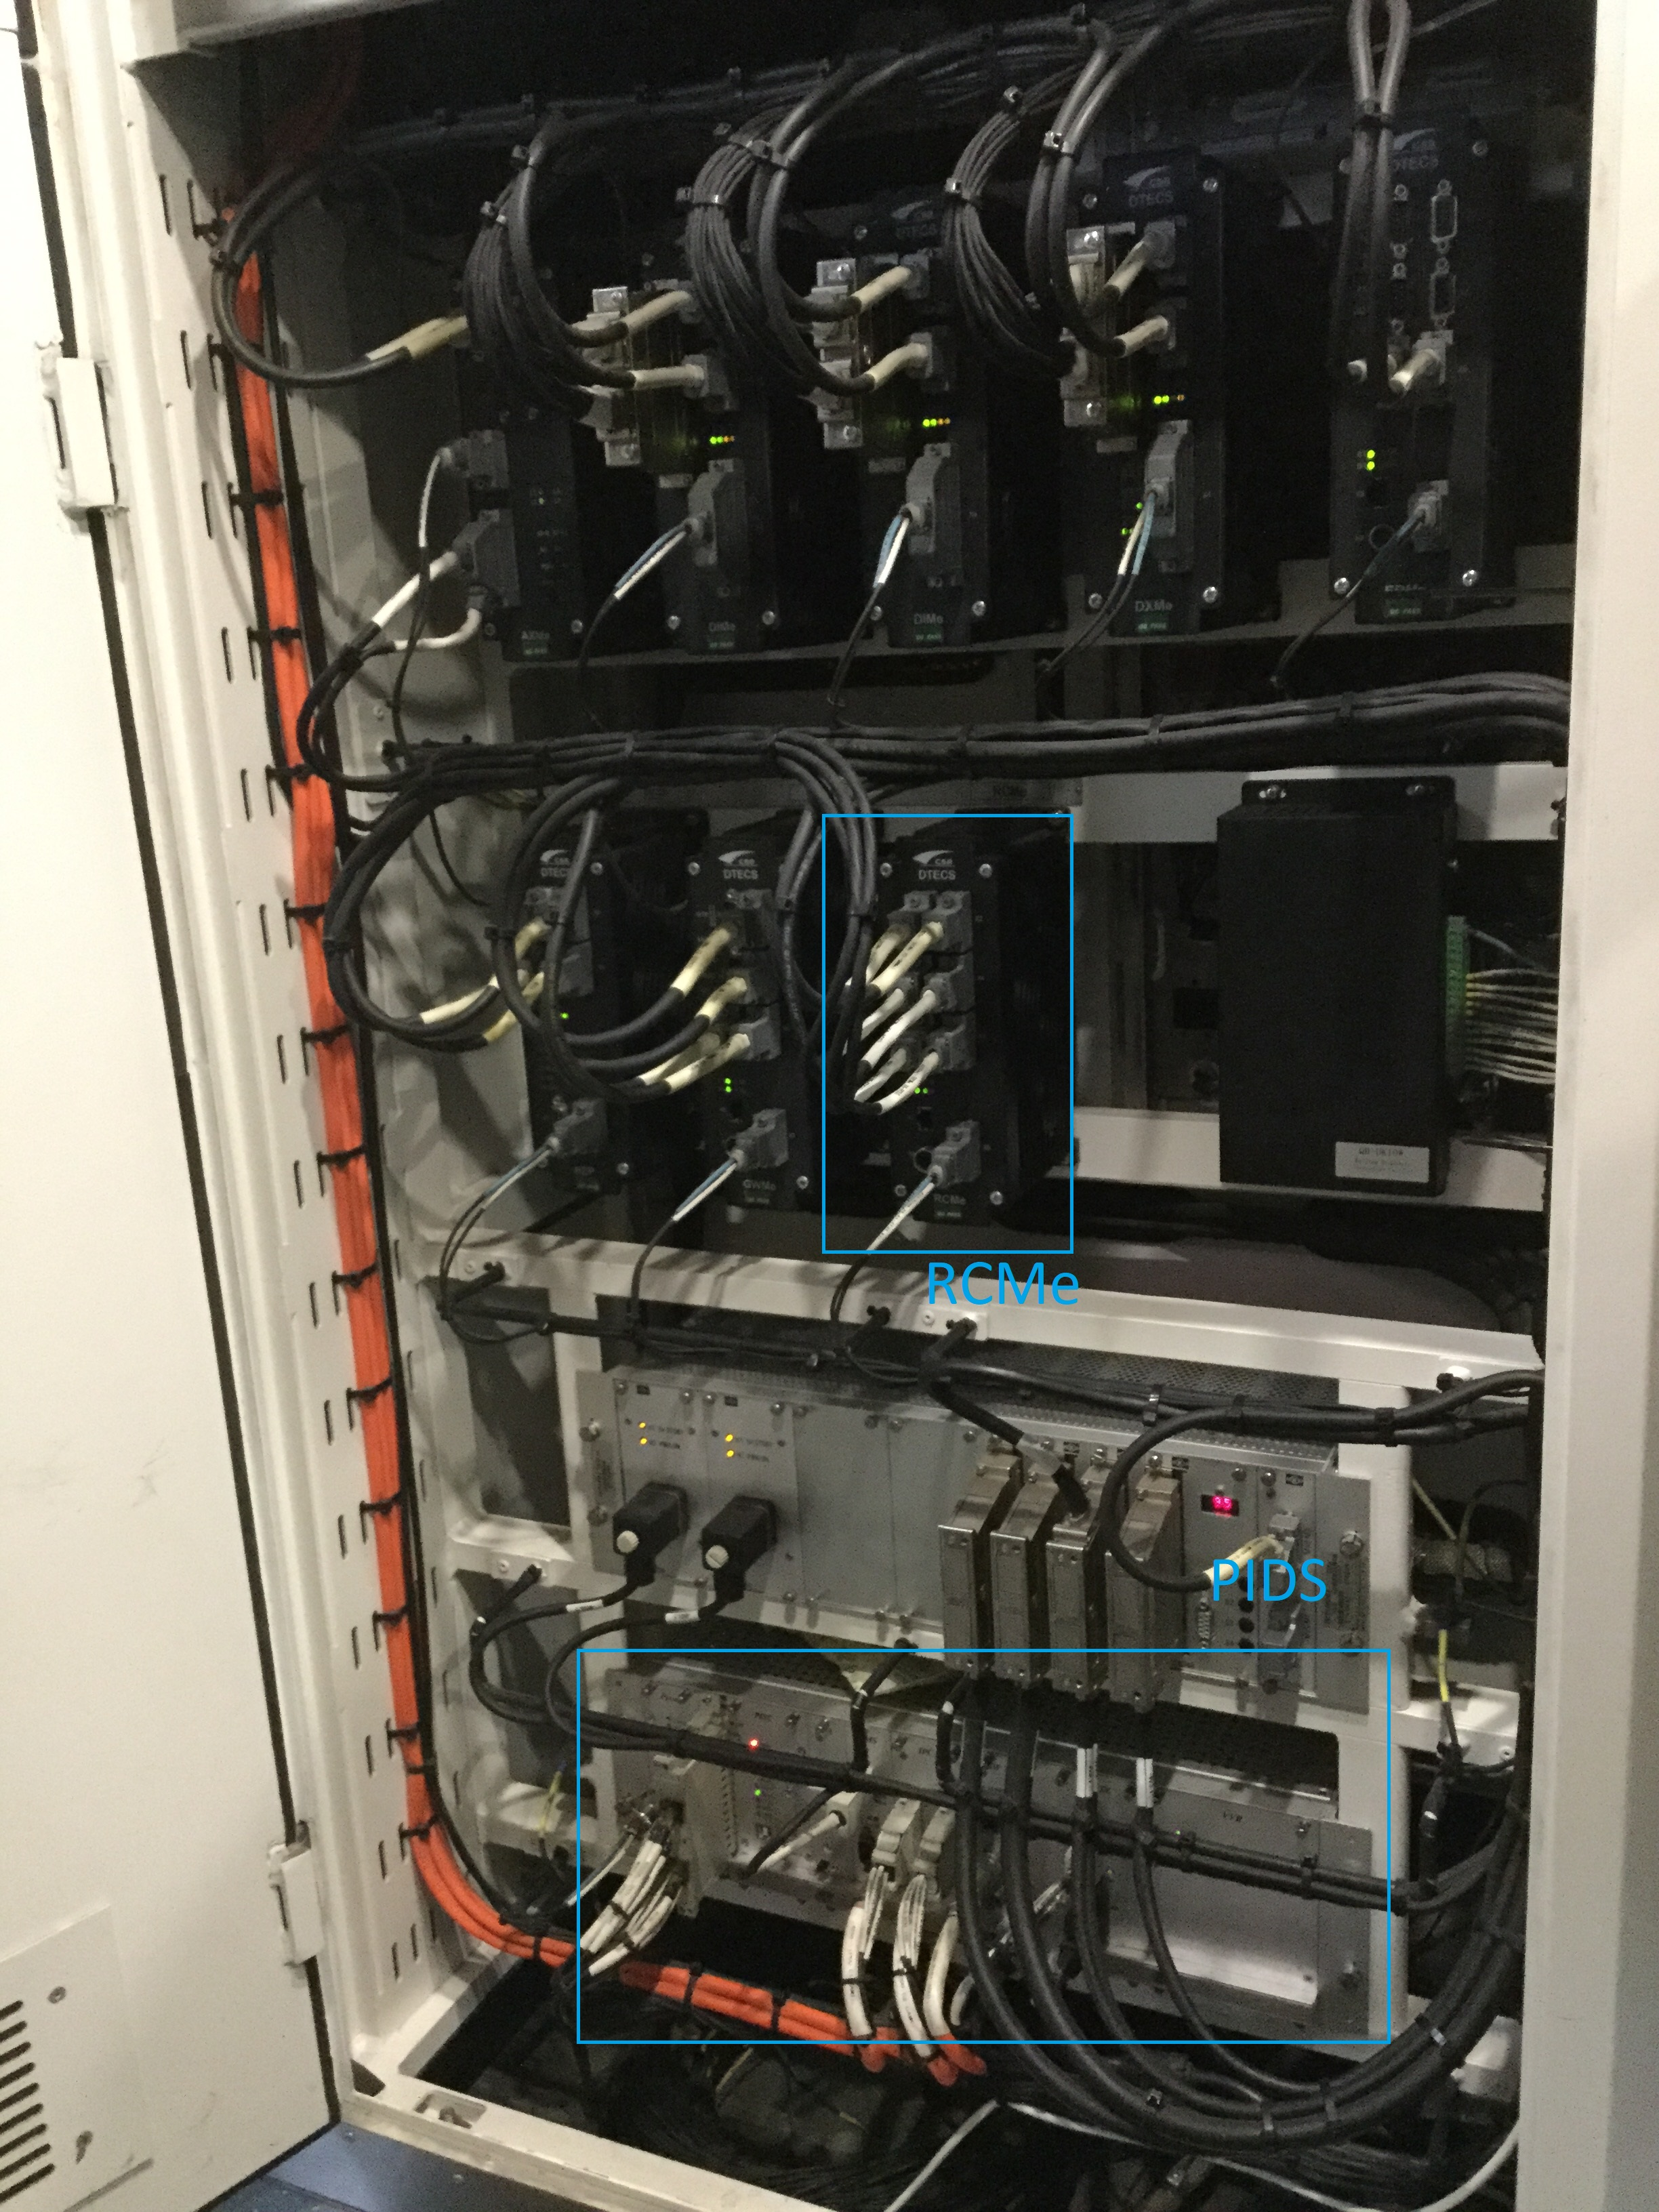
\includegraphics[width=0.5\textwidth , angle=0]{./Figures/imgRackTCN.JPG}
	\caption{Fotografía del rack de salón de una formación de Trenes Argentinos.}
	\label{fig:imgRackTCN}
\end{figure}

En conjunto, estos módulos negros DIMe, DXMe, RCMe, son parte de la solución para TCN del Instituto Zhuzhou, denominada Distribute Train Electric Control System (DTECS)  \cite{feng2016survey}. Los módulos incluyen un gateway WTB/MVB. Se ha observado en las formaciones de trenes y también en el plano de la red TCN que el sistema PIDS tiene su propia red RS485. En la figura \ref{fig:rackPIDS1} se muestra un detalle de la unidad de rack con los módulos del sistema PIDS.\\

\begin{figure}[h!]
	\centering
	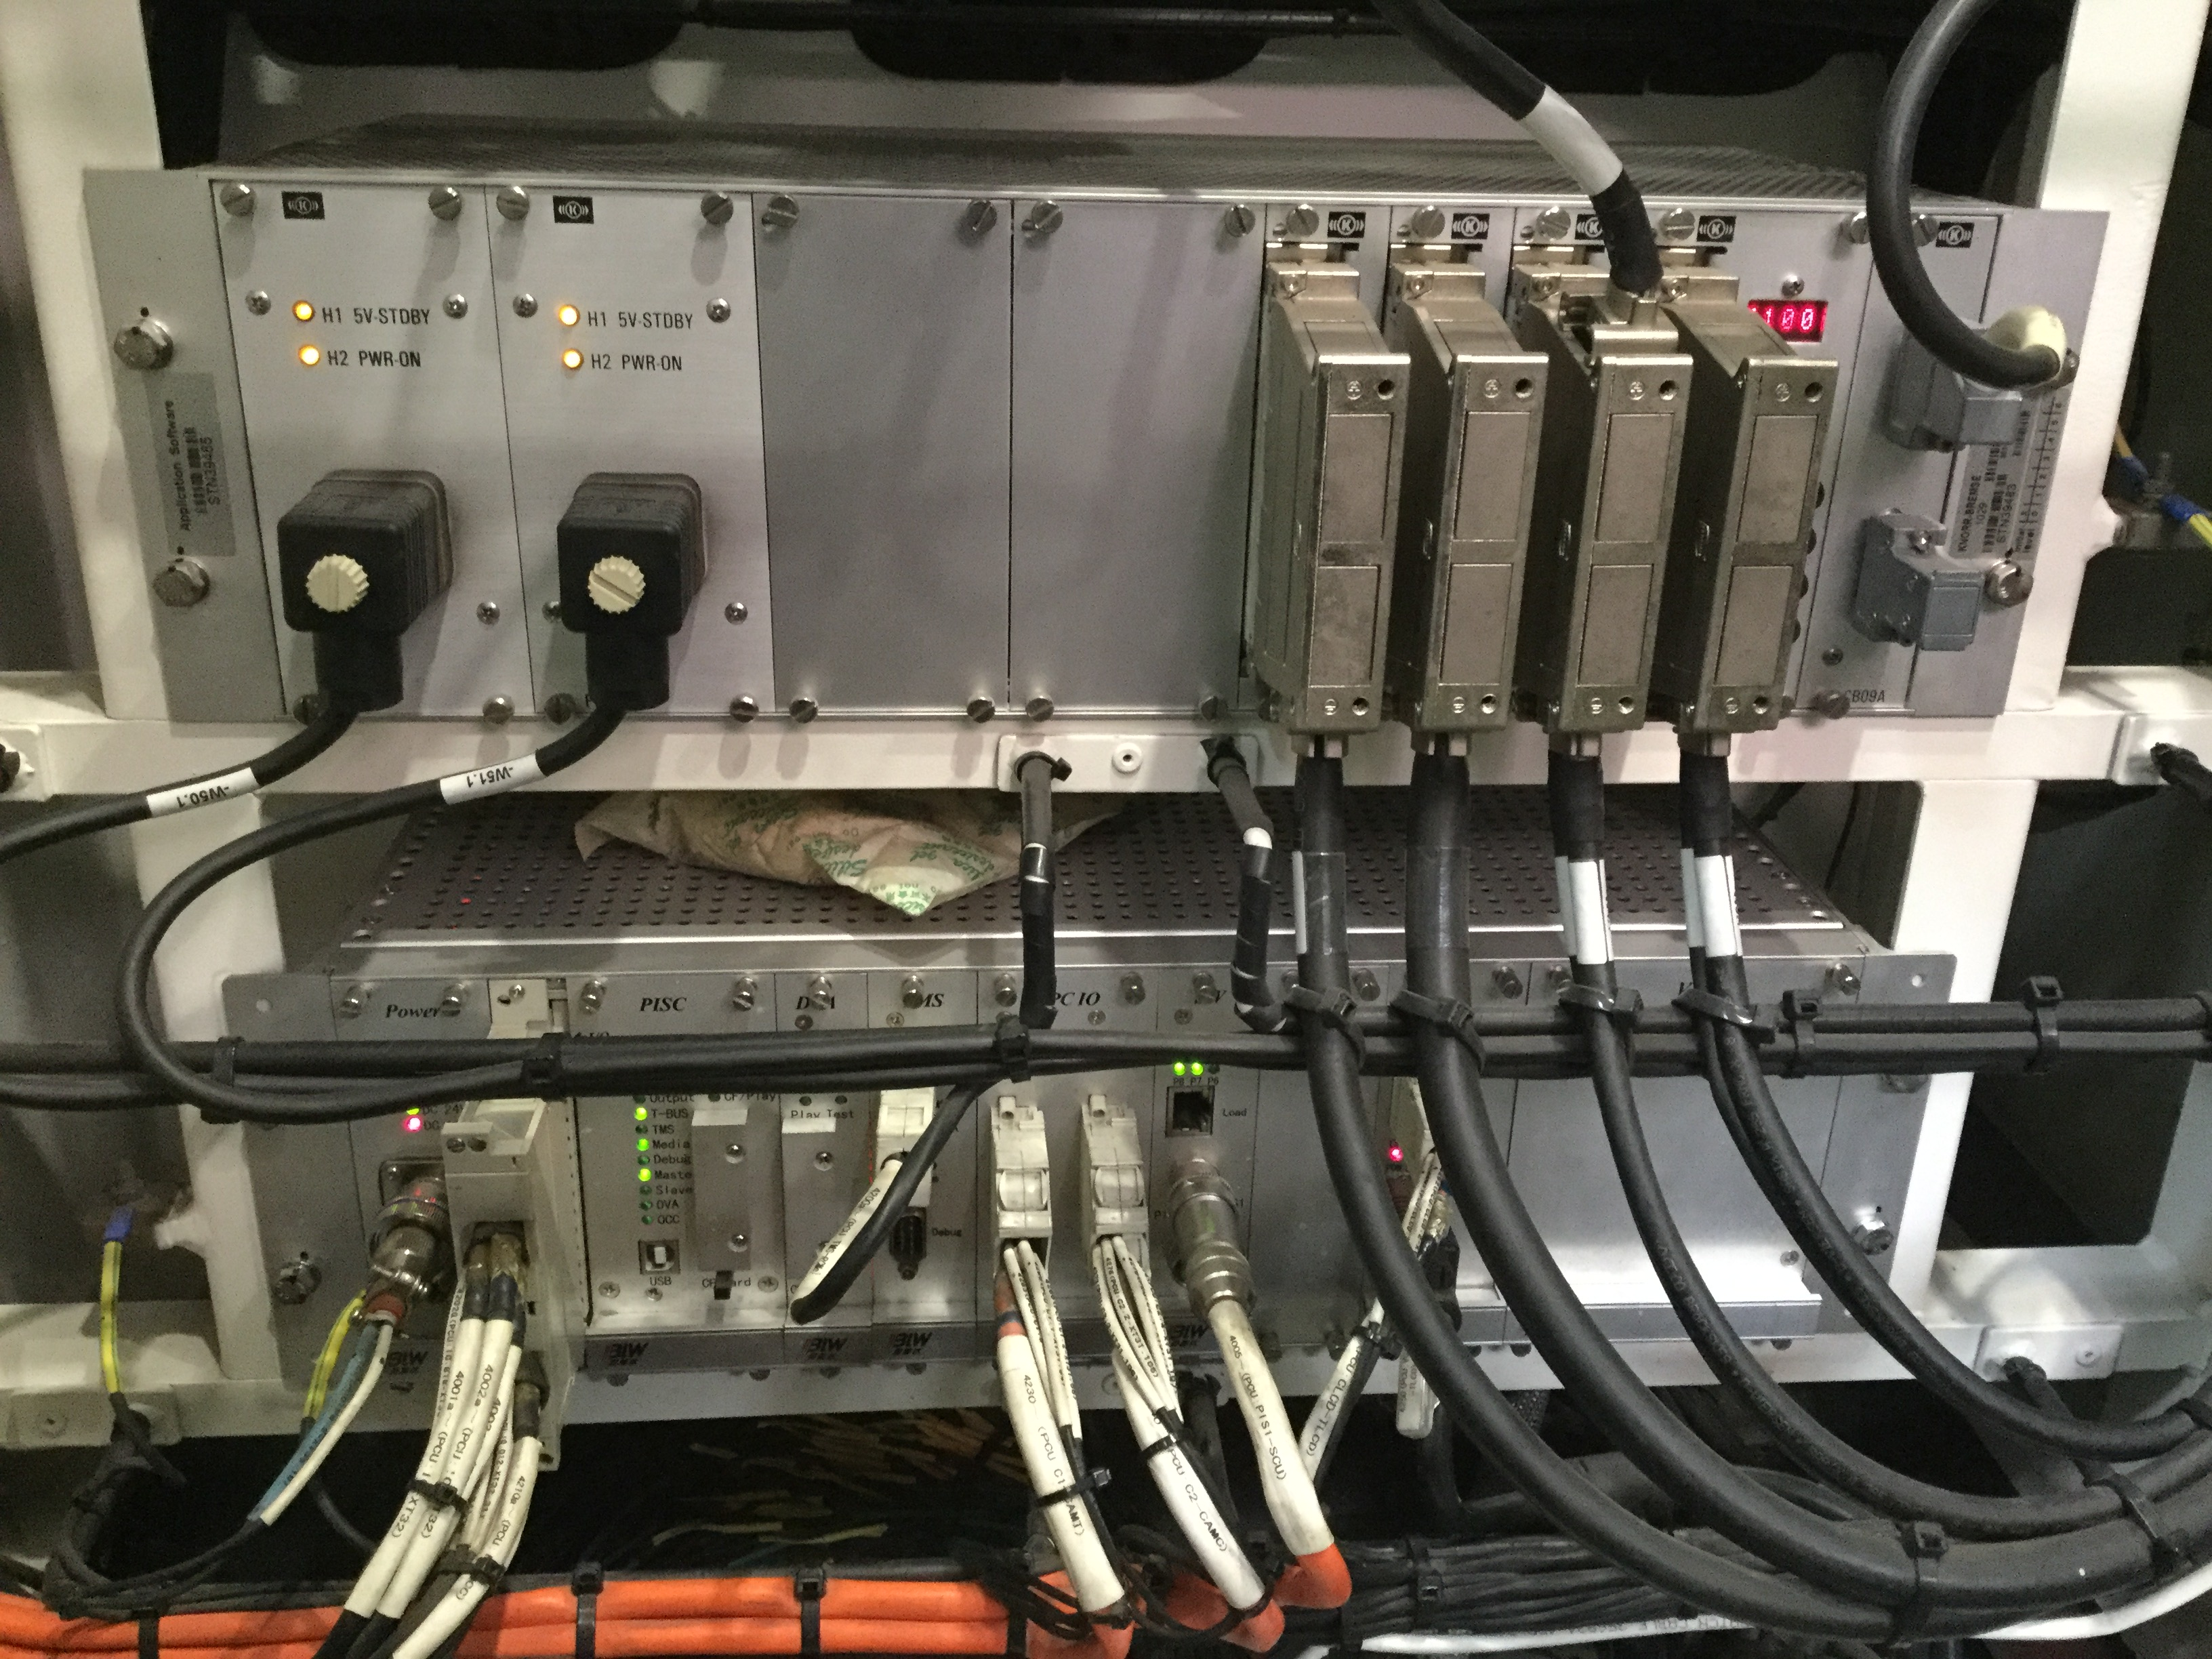
\includegraphics[width=0.5\textwidth]{./Figures/rackPIDS1.JPG}
	\caption{Fotografía de las unidades de rack del sistema PIDS en el rack de salón.}
	\label{fig:rackPIDS1}
\end{figure}

En el sistema PIDS propietario también se incluyen otros módulos que se detallan en la siguiente sección.


\section{PIDS: Sistema de información visual para pasajeros}

El sistema de información al pasajero existente en las formaciones relevadas no sigue un estándar, sino que es una solución propietaria para resolver el circuito de cámaras, el sistema de audio, los mapas de recorrido y los carteles LED. En la figura \ref{fig:diagramaPIDS} se presenta la arquitectura del sistema PIDS propietario existente en las formaciones de SOFSE.\\

\begin{figure}[h!]
	\centering
	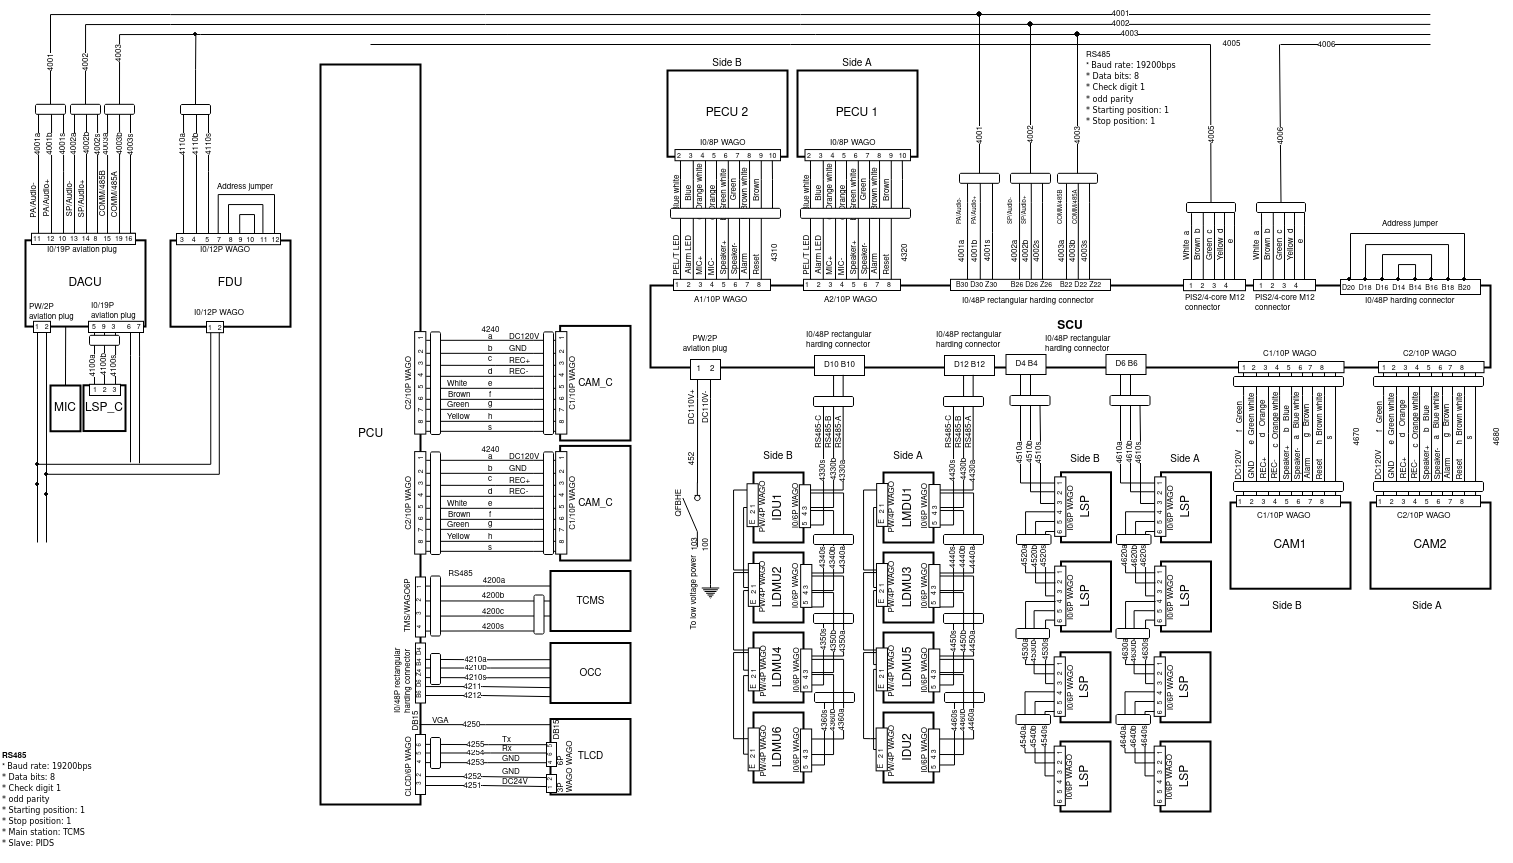
\includegraphics[width=1.5\textwidth, angle=90]{./Figures/diagramaPIDS.png}
	\caption{Diagrama de bloques del sistema PIDS, elaborado por el autor en base al plano de referencia de SOFSE.}
	\label{fig:diagramaPIDS}
\end{figure}

Este plano de referencia detalla importantes conexiones del sistema. Leyendo de izquierda a derecha, se pueden observar dos módulos denominados DACU y FDU, encargados del micrófono, del audio, de comunicarse a través del módulo vertical PCU  con los sistemas CAM T, CAM C, TCMS, OCC y TLCD (pantalla LCD del conductor) y de ser un extremo de conexión del bus de datos RS485 a través del cableado 4001, 4002 y 4003. Este bus se interconecta a un módulo horizontal denominado SCU al que se conectan otra serie de módulos: PECU1 y PECU2 indicando referencia de los laterales del tren, CAM1 y CAM2, y cuatro arreglos serie de módulos. Dos de los módulos serie integran los bloques IDU (carteles de matriz led) y LDMU (mapas de recorrido led). Los otros dos módulos serie integran los bloques LSP o parlantes. Se puede observar que de estas conexiones serie hay dos módulos IDU: IDU1 al comenzar y IDU2 al finalizar el arreglo serie. Esto se corresponde con la distribución espacial de los carteles de matriz led en el salón de cada coche.\\



\section{Carteles y controladoras de matrices LED}

